\subsection{Lab2: Osciloscopio y FFT}
%*********************
\begin{frame}{}

\pgfdeclareimage[width=\paperwidth,height=\paperheight]{bg}{imagenes/fondo_lab}
\setbeamertemplate{background}{\pgfuseimage{bg}}

\bfseries{\textrm{\LARGE Lab2\\ \Large Osciloscopio y FFT}}
\raggedright
\end{frame}
%*********************

%-----------------------------------
\begin{frame}{Osciloscopio y FFT\index{TCP}}

\pgfdeclareimage[width=\paperwidth,height=\paperheight]{bg}{imagenes/fondo3}
\setbeamertemplate{background}{\pgfuseimage{bg}}

En este laboratorio se genera una onda senoidal y a su vez algún ruido; estas dos señales se suman y se observa el resultado en el dominio de la frecuencia (FFT) y del tiempo (Scope). Se aprende a utilizar el notebook y algunas herramientas básicas del GRC. 

\end{frame}
%---------------------------------

\begin{frame}{Osciloscopio y FFT\index{TCP}}

\begin{figure}[H]
\vspace{-4mm}
\centering
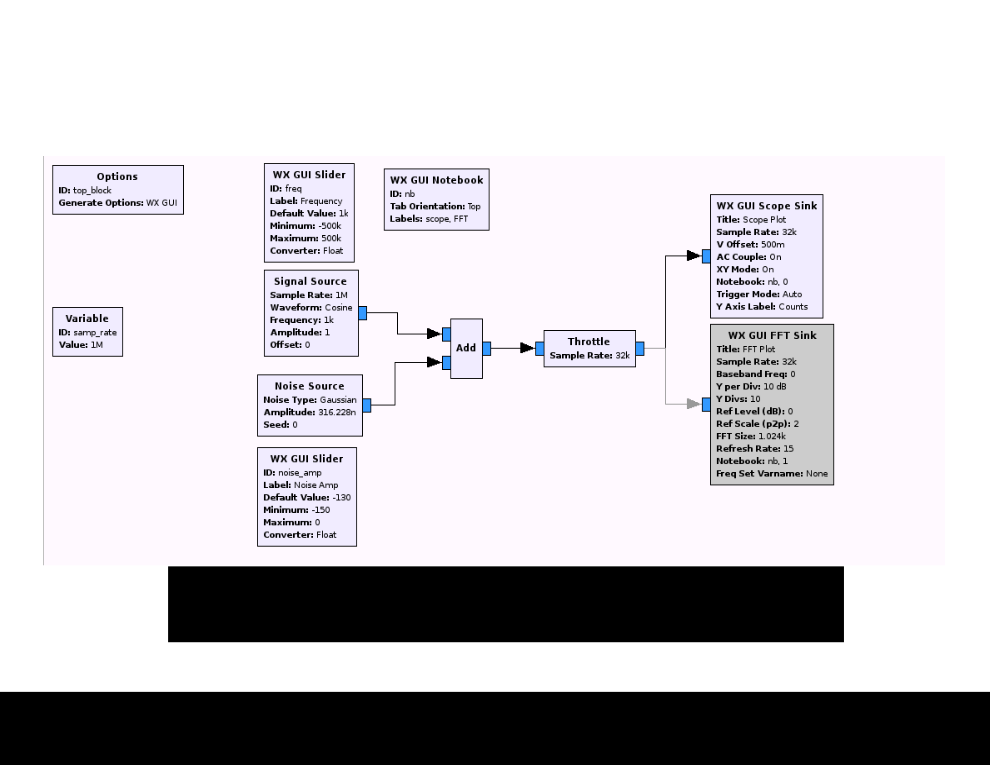
\includegraphics[width=1.2\textwidth]{parte1/lab2/pdf/lab2_1.pdf}
\end{figure}
\end{frame}
%---------------------------------

\begin{frame}{Osciloscopio y FFT}
\begin{figure}[H]
\vspace{-4mm}
\centering
\includegraphics[width=1.1\textwidth]{parte1/lab2/pdf/lab2_2.pdf}
\end{figure}
\end{frame}
%--------------------------------

\begin{frame}{Osciloscopio y FFT\index{Noise Source}}
\begin{figure}[H]
\centering
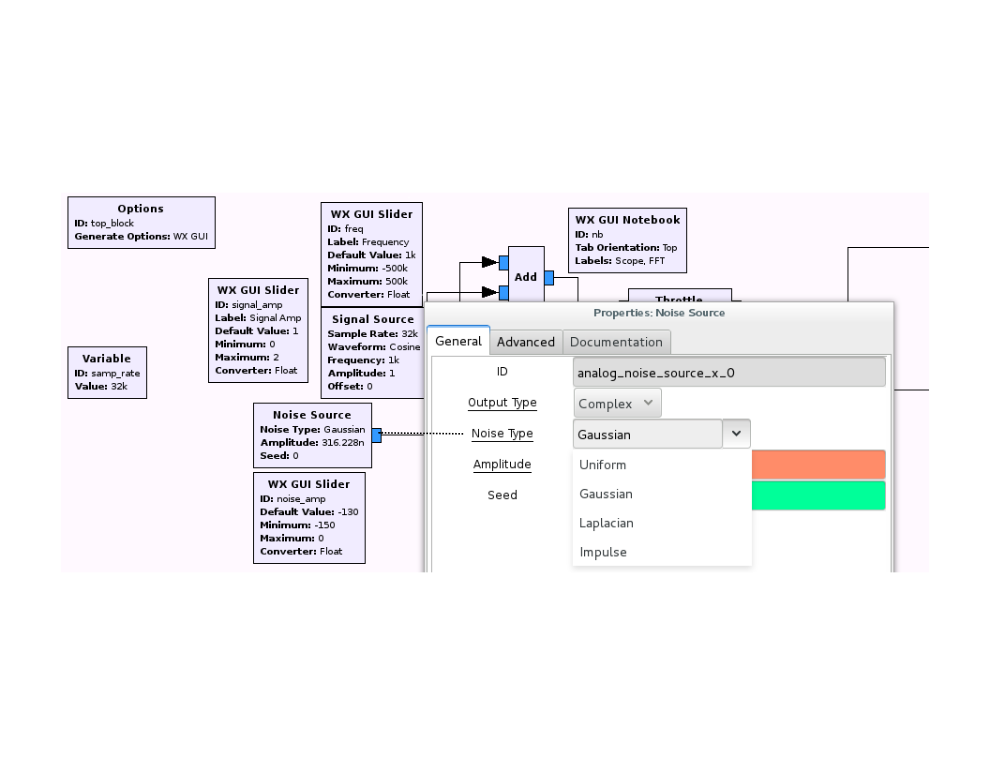
\includegraphics[width=1.055\textwidth]{parte1/lab2/pdf/lab2_3.pdf}
\end{figure}
\end{frame}
%--------------------------------

\begin{frame}{Osciloscopio y FFT\index{Noise Source}}
\begin{figure}[H]
\centering
\includegraphics[width=1.055\textwidth]{parte1/lab2/pdf/lab2_4.pdf}
\end{figure}
\end{frame}
%--------------------------------

\begin{frame}{Osciloscopio y FFT\index{Add}}
\begin{figure}[H]
\centering
\includegraphics[width=.7\textwidth]{parte1/lab2/pdf/lab2_5.pdf}
\end{figure}
\end{frame}
%--------------------------------

\begin{frame}{Osciloscopio y FFT}
\begin{figure}[H]
\vspace{-4mm}
\centering
\includegraphics[width=1.1\textwidth]{parte1/lab2/pdf/lab2_6.pdf}
\end{figure}
\end{frame}
%--------------------------------

\begin{frame}{Osciloscopio y FFT\index{WX GUI Notebook}}
\begin{figure}[H]
\vspace{-4mm}
\centering
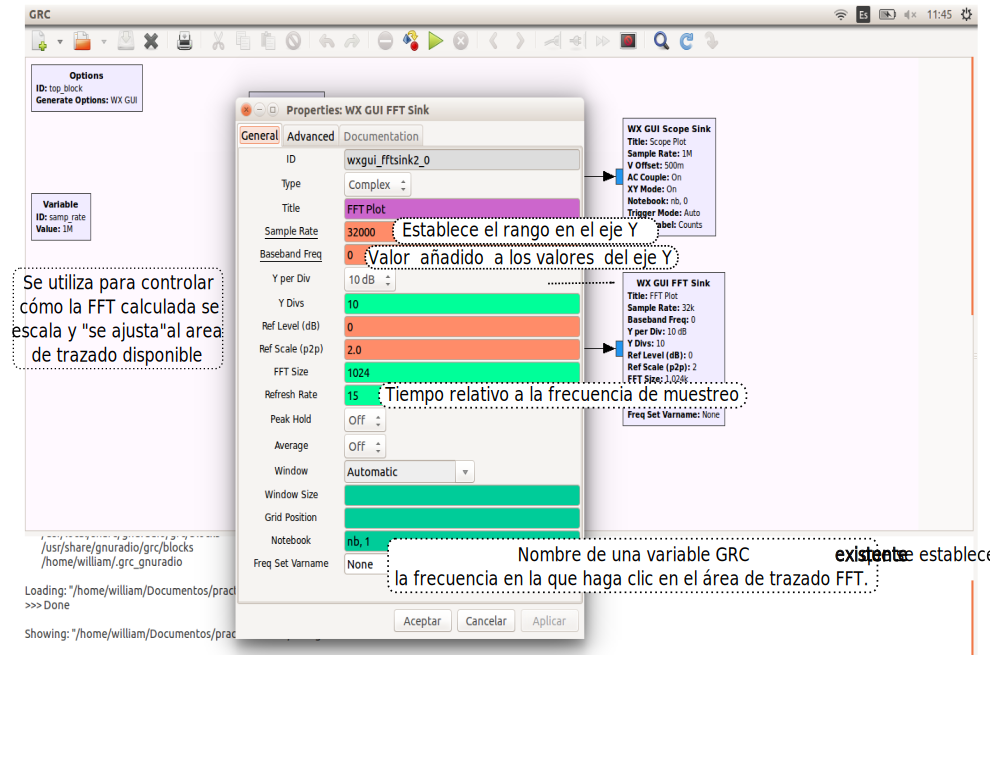
\includegraphics[width=0.85\textwidth]{parte1/lab2/pdf/lab2_7.pdf}
\end{figure}
\end{frame}
%--------------------------------

\begin{frame}{Osciloscopio y FFT\index{WX GUI FFT Sink}}
\begin{figure}[H]
\centering
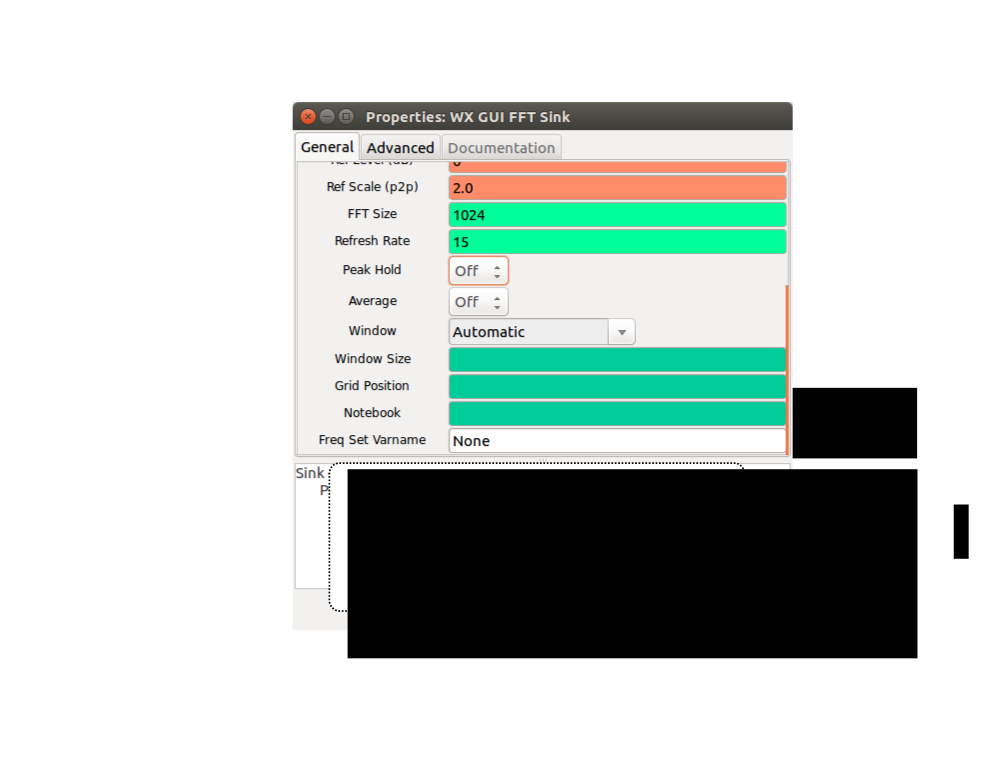
\includegraphics[width=1.1\textwidth]{parte1/lab2/pdf/lab2_8.pdf}
\end{figure}
\end{frame}
%--------------------------------

\begin{frame}{Osciloscopio y FFT\index{WX GUI FFT Sink}}
\begin{figure}[H]
\vspace{-3mm}
\centering
\includegraphics[width=0.7\textwidth]{parte1/lab2/pdf/lab2_9.pdf}
\end{figure}
\end{frame}
%--------------------------------

\begin{frame}{Osciloscopio y FFT}
\begin{figure}[H]
\vspace{-3mm}
\centering
\includegraphics[width=0.85\textwidth]{parte1/lab2/pdf/lab2_10.pdf}
\end{figure}
\end{frame}
%--------------------------------

\begin{frame}{Osciloscopio y FFT}
\begin{figure}[H]
\vspace{-3mm}
\centering
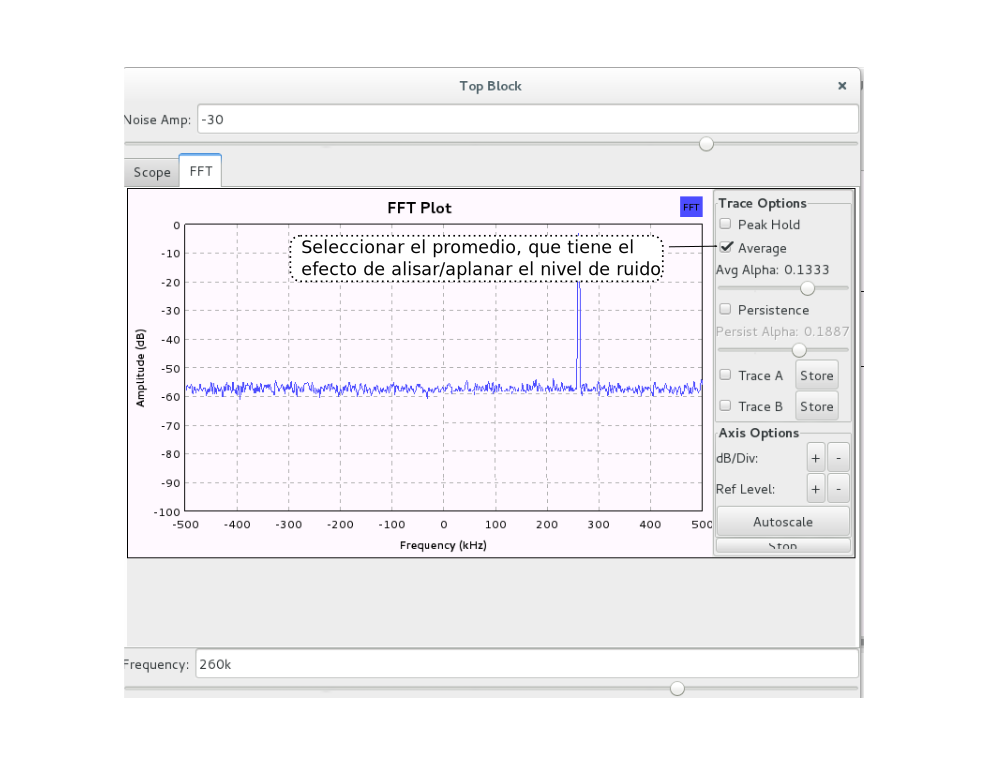
\includegraphics[width=0.75\textwidth]{parte1/lab2/pdf/lab2_11.pdf}
\end{figure}
\end{frame}
%--------------------------------

\begin{frame}{Osciloscopio y FFT}
\begin{figure}[H]
\vspace{-3mm}
\centering
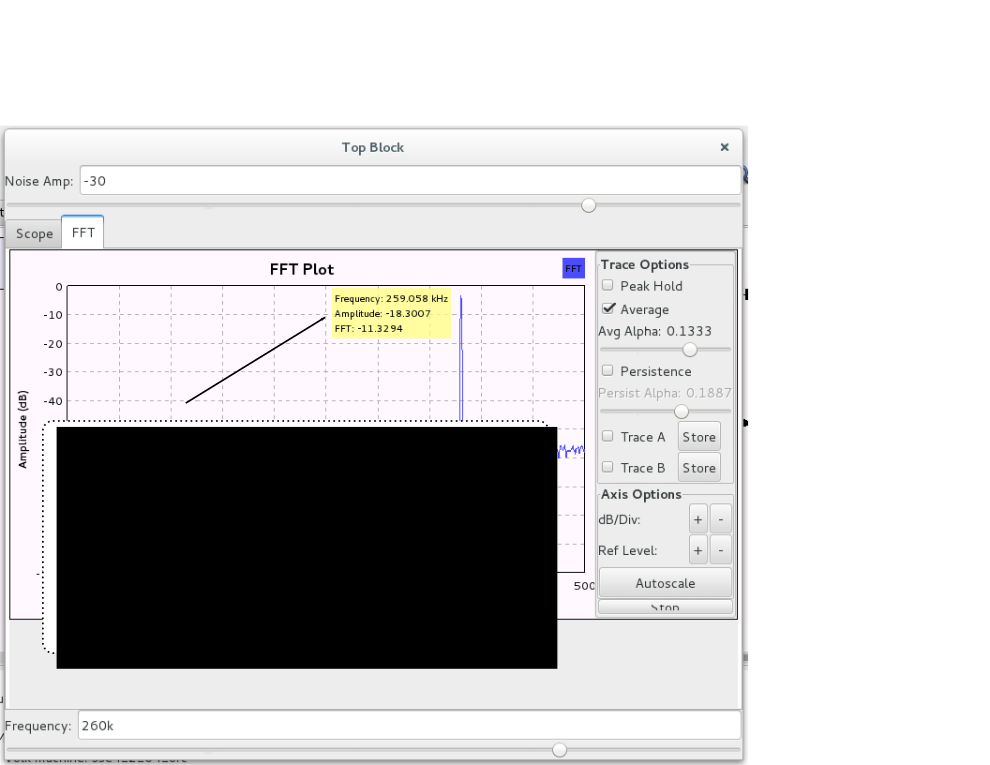
\includegraphics[width=0.75\textwidth]{parte1/lab2/pdf/lab2_12.pdf}
\end{figure}
\end{frame}
%--------------------------------

\begin{frame}{Osciloscopio y FFT}
\begin{figure}[H]
\centering
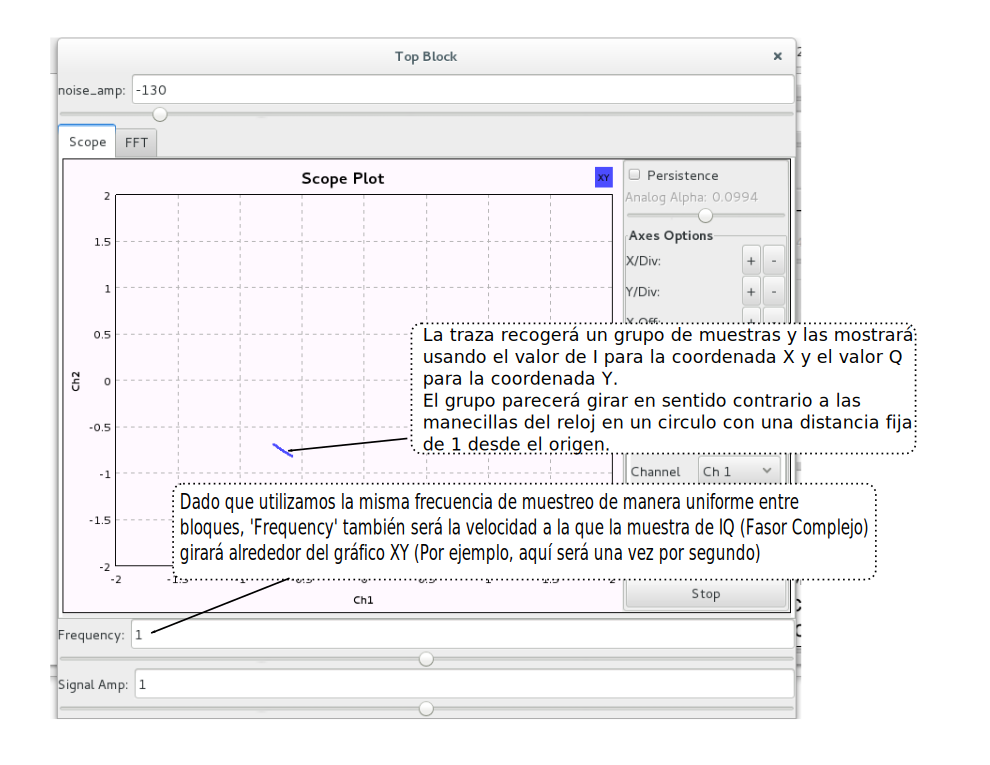
\includegraphics[width=0.75\textwidth]{parte1/lab2/pdf/lab2_13.pdf}
\end{figure}
\end{frame}
%--------------------------------

\begin{frame}{Osciloscopio y FFT}
\begin{figure}[H]
\vspace{-3mm}
\centering
\includegraphics[width=0.75\textwidth]{parte1/lab2/pdf/lab2_14.pdf}
\end{figure}
\end{frame}
%--------------------------------

\begin{frame}{Osciloscopio y FFT}
\begin{figure}[H]
\vspace{-3mm}
\centering
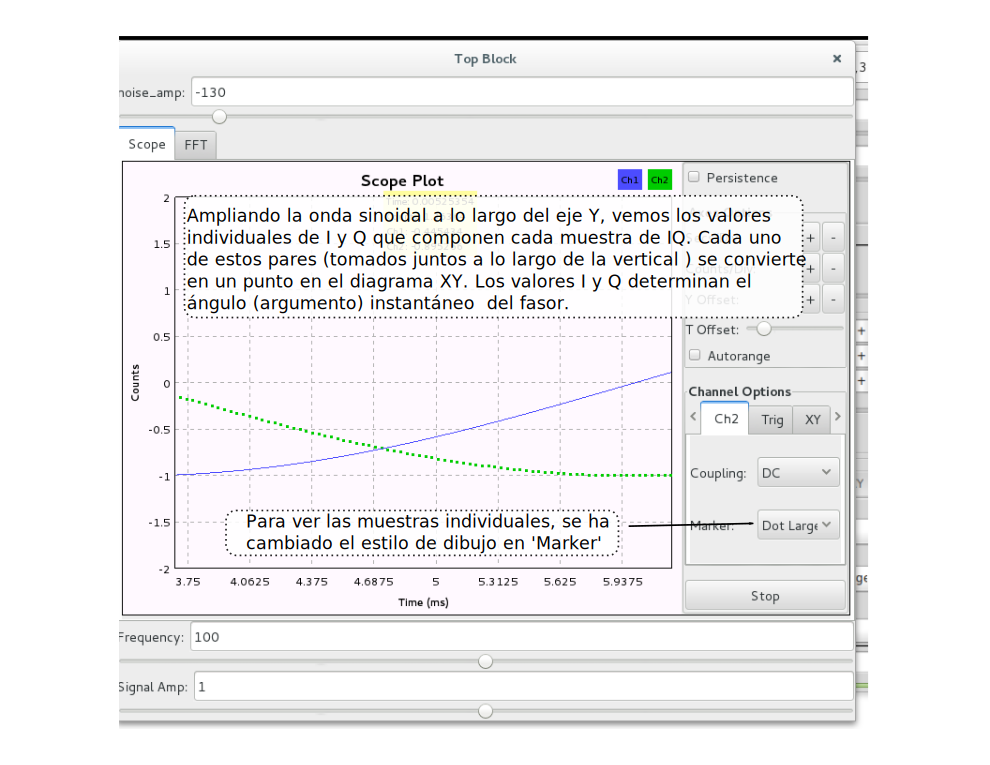
\includegraphics[width=0.7\textwidth]{parte1/lab2/pdf/lab2_15.pdf}
\end{figure}
\end{frame}
%--------------------------------

\begin{frame}{Osciloscopio y FFT}
\begin{figure}[H]
\centering
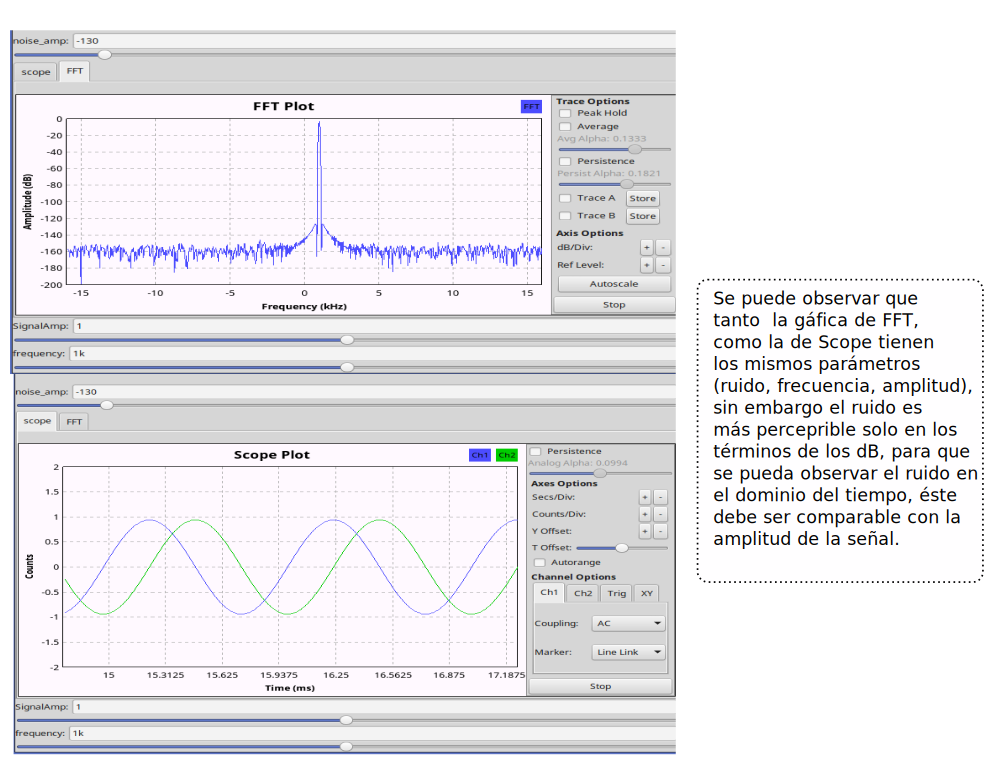
\includegraphics[width=\textwidth, height=0.58\textwidth]{parte1/lab2/pdf/lab2_16.pdf}
\end{figure}
\end{frame}
%--------------------------------

%\usepackage{amssymb}
%\usepackage{amsmath}
\subsubsection{Actividad 1 lab 2}
%*********************
\begin{frame}{}

\pgfdeclareimage[width=\paperwidth,height=\paperheight]{bg}{imagenes/fondo_seccion}
\setbeamertemplate{background}{\pgfuseimage{bg}}

\definecolor{greenU}{RGB}{212,202,72}
\setbeamercolor{block body}{fg=Black,bg=greenU}
\begin{block}{}
	\centering
	\vspace{1mm}
	\large{\textit{Actividades}}
	\vspace{1mm}
\end{block}
\end{frame}
%*********************


%--------------------------------
\begin{frame}{Actvidad 1 lab 2}
\begin{figure}[H]
\begin{flushleft}
Mencione los diferentes tipos de ruido del bloque (noise source), sus características,
describa la función de densidad de probabilidad para cada uno de estos y por que se puede ocasionar
\end{flushleft}
\centering
\includegraphics[width=\textwidth, height=0.58\textwidth]{parte1/lab2/pdf/lab2_17.pdf}
\end{figure}
\end{frame}
%--------------------------------


\subsubsection{Actividad 2 lab 2}
%*********************

\begin{frame}{Actvidad 2 lab 2}
\begin{figure}[H]
\begin{flushleft}
Objetivos:
\end{flushleft}
\begin{flushleft}
-Dar a conocer a lector la distribución  de los diferentes tipos de ruido y sus propiedades.
\end{flushleft}
\begin{flushleft}
-Relacionar las funciones de densidad con cada uno de los diferentes ruidos que aparecen en el modulo noise source.
\end{flushleft}
\begin{flushleft}
-Mediante una breve configuración al lab 2 compare y evidencie que lo anterior se cumpla.
\end{flushleft}

\begin{center}
\centering
\includegraphics[width=\textwidth, height=0.58\textwidth]{parte1/lab2/pdf/lab2_18.pdf}
\end{center}
\end{figure}
\end{frame}
%--------------------------------

\subsubsection{Actividad 2 lab 3}
%*********************
%--------------------------------
\begin{frame}{Actvidad 3 lab 2}
\begin{figure}[H]
\begin{flushleft}
Objetivo:
\end{flushleft}
\begin{flushleft}
-Variar la  amplitud y fase de la señal para generar las curvas de Lissajous.
\end{flushleft}

\begin{center}
\centering
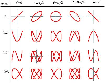
\includegraphics[width=0.65\textwidth]{parte1/lab2/pdf/lab2_19.pdf}
\end{center}
\end{figure}
\end{frame}
%--------------------------------
